\chapter{实现}

本章整理总结系统实现过程中遇到的关键问题的解决方案以及解决问题的过程中进行的探索性过程。\footnote{考虑到表述紧凑性,本章节仅包含描述解决方案所必须的代码片段,详细的代码实现请参考附录内的相关内容}

\section{开发环境与技术选择}

系统开发主要使用 JavaScript 语言平台,应用服务器端使用 Node.js 而客户端使用 JavaScript 脚本开发业务代码。

\begin{figure}[!h]
  \begin{center}
    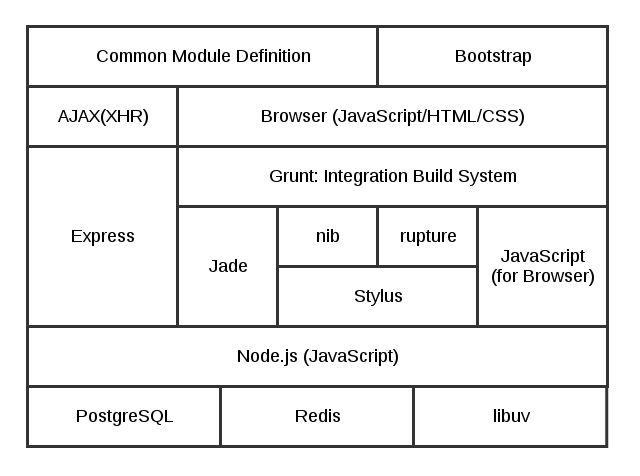
\includegraphics[width=\textwidth]{figures/diagram-tech-stack.png}
    \caption{开发环境与外部组件\label{TechStack}}
  \end{center}
\end{figure}

相较 Java/.NET 等流行的企业级解决框架,Node.js 支持函数式编程范式,在 Express 框架的帮助下可以快速的搭建稳定的服务器应用。另外,选择 Node.js 的一大原因是 Node.js 采用消息队列机制,并支持异步 I/O 操作,单线程异步操作模型可以有效的减少内存开销,同时,避免了传统服务器开发过程中所容易出现的线程同步问题,极大的提升了服务器的稳定性。对轻量服务器设计来说使用 Node.js 能够在取得良好的服务器性能以及稳定性的同时达到最大的开发效率。

客户端代码使用 Grunt 集成编译系统进行独立编译,相比使用 Express 进行线上编译-缓存的策略,使用 Grunt 集成编译环境直接将客户端程序编译为线上版本有利于前端服务器直接对文件进行缓存操作,将客户端资源编译工作从应用服务器中分离出来也有利于应用服务器自身的可扩展性和运行时性能。

\section{服务器(Model)}

应用服务器的职能在系统中主要负责多用户会话维护、权限控制以及数据操作。

\subsection{轻量级 Object-Relation Mapping 实现}

Object-Relation Mapping (ORM) 是将数据库关系与数据库实体的数据直接通过面向对象封装进行访问的一种方法。

服务器对数据库的业务访问逻辑普遍包含:

\begin{itemize}
  \item 验证业务数据有效性
  \item 转换业务数据(如 进行 Password Hash)
\end{itemize}

为了提高数据库访问代码的复用程度,项目中设计了 $querybuilder$ 轻量级数据库 ORM 框架,以用户资料管理为例:

\begin{verbatim}

        profile: {

          update: qb('INSERT INTO profile SET ? ON DUPLICATE KEY UPDATE ?', {
            user_id : Number,
            name    : String,
            gender  : String
          }),

          query: qb([
            'SELECT a.`user_id` AS `user_id`,',
            '       p.`name`    AS `name`, ',
            '       p.`gender`  AS `gender`,',
            'FROM `account` a INNER JOIN `profile` p ON a.user_id = p.user_id',
            'WHERE a.`account` = :account AND a.`domain` = :domain'
          ].join(' '), { account: String, domain: String })

        },

\end{verbatim}

$qb$ 函数返回用于数据库查询的高阶函数,在中间件中:

\begin{verbatim}

        db.profile.update(req.data, function (err, result) {

          if (err) {
            return next(new ApplicationError({
              message: 'Failed to update user profile',
              cause: err
            }));
          }

          return res.status(200).end();

        });

\end{verbatim}

通过使用简单的 ORM 框架,对 SQL 语句模板进行集中统一的管理,让业务逻辑代码得到了高效的组织。

\subsection{权限控制中间件}

中间件是 Express.js 服务器框架所使用的基本设计模式。

\begin{figure}[!h]
  \begin{center}
    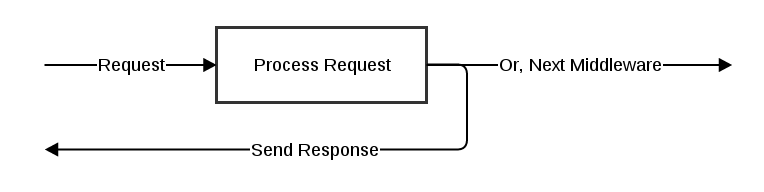
\includegraphics[width=\textwidth]{figures/diagram-express-middleware.png}
    \caption{中间件行为示意图\label{ExpressMiddleware}}
  \end{center}
\end{figure}

获得请求以后 Express.js 会按照中间件的注册顺序使用中间件处理请求,中间件返回三种处理结果:

\begin{enumerate}
  \item 处理完成,发送响应数据
  \item 进行数据变换,发送至下一个中间件
  \item 处理失败,使用错误处理中间件进行处理
\end{enumerate}

权限控制中间件用于实现服务器接口的权限控制(见~\ref{sec:ServerAPI})。

权限控制中间件通过传入的高阶函数判断当前对接口进行的请求的合法性:

\begin{verbatim}

        app.post('/c/:id/t/',
          // role of current user is admin or teacher
          accessctl(role('admin'), role('teacher')),
          // can access c of :id with current request
          accessctl(from('/c/:id/', 'c')),
          function (req, res, next) {
            // Bussiness code
          }
        )

\end{verbatim}

上面的例子中 $role$ 与 $from$ 分别是用于确认用户角色以及其他接口访问能力的~\textbf{权限策略},$accessctl$ 通过执行权限策略并检查策略的执行结果决定是否给予当前的请求进行下一步中间件。

除了应用于对某个接口的权限控制,$accessctl$ 还可以通过 $express.use$ 方法配置一组 $router$ 的权限。

\section{客户端视图模型(ViewModel)}

项目中使用 Monad 对 MVVM 模式中 ViewModel 进行实现,替代面向对象设计中的 Observer 模式。Monad 与 Observer 都能合理的组织代码,将代码复杂度保持在线性增长的状态,而 Monad 在函数式开发环境中更容易实现和使用。

本项目尝试开发的 Entangle 框架经过三次迭代最终满足客户端前端开发的需求,Entangle 框架使用 Monad 作为 Reactive Programming 的响应核心,并在此基础上封装 Builder 模式以简化对业务逻辑中经常出现的顺序逻辑的定义过程。下面几个小节对 Entangle 框架成型过程中所解决的重要业务需求以及其实现方案进行叙述。

\subsection{数据同步}

与服务器进行数据交互是客户端的基础功能之一。

通过 $http$ 转换子(Converter)实现从服务器拉取数据:

\begin{verbatim}

        entangle().http('GET', '/u').pick(function (data) { /* ... */ });

\end{verbatim}

Entangle 使用链式表达式构建串行关系的转换子(Converter),上例实现获取用户信息的功能。

对于轮询的情况,可以使用 $timeout$ 转换子:

\begin{verbatim}

        var juice = entangle().http('GET', '/u')
        var timer = entangle().timeout(2000);

        timer.fork(juice);
        juice.fork(timer);

\end{verbatim}

$fork$ 原语将 timer 的值转发到 juice,当 timer 触发时,触发事件会传递给 juice、发出 http 请求,请求完成后 juice 又会将数据 fork 回 timer 进行下一个 $2s$ 的等待。这样就造成了一个轮询的数据流。

详细的实现请参考附录内容,在这里我们不详细展开 Entangle 的实现细节。

\subsection{页面导航}

页面导航栏的逻辑是单一对象数据绑定的比较典型的实现。entangle 通过自动改写的 jQuery 方法实现对用户界面元素的操作,下面这些代码来自 pilot.js:

\begin{verbatim}

        entangle()
        .location()
        .pick().string('.navbar-collapse a[href="{{pathname}}"]')
        .$().$parent('li').$addClass('active')

\end{verbatim}

$string$ 转换子将输入的数据代入字符串模板,$\$$ 转换子将输入的字符串转换为 jQuery 对象之后以 \$ 开始的转换子都经过自动改写指向对应的 jQuery 方法。

$location$ 转换子实现对页面地址信息的监听:

\begin{verbatim}

        location: function () {

          var converter = function () {
            this.resolve(location);
          };

          // get location from window object
          var location = {
            host: window.location.host,
            hostname: window.location.hostname,
            protocol: window.location.protocol,
            search: window.location.search,
            href: window.location.href,
            port: window.location.port,
            pathname: window.location.pathname,
            hash: window.location.hash,
          };

          // listen for hash change event
          $(window).on('hashchange', function () {
            location.hash = window.location.hash;
            converter.resolve(location);
          });

          return converter;

        }

\end{verbatim}

这里介绍一下转换子的构成:

\begin{itemize}
  \item 转换子是一个返回高阶函数的函数
  \item 转换子内可以定义自己的闭包状态
  \item 转换子可以进行事件监听
  \item 转换子使用 $resolve$ 方法将数据传输给后继转换子
\end{itemize}

另外,这里需要特别说明的问题是,基础的转换子实现是基于面向过程的编程方法的,事实上 Haskell 在描述具体的“怎么做”(HOW)逻辑的时候也使用 $do$ 语法糖模拟顺序执行的代码(通过参照代码行之间的前后依赖关系,在定义“是什么”(WHAT)的情况下依赖关系是由“是什么”定义的,不参照代码行的前后依赖关系),这也是支持混合语言特性的语言的优势所在。

\subsection{绑定列表数据}

第三版的 entangle 对列表数据的绑定做出了设计,第二版 entangle 中使用 entangle 核心对上下文进行切换管理,这样做所产生的代价是核心代码的大量冗余与不可扩展性,因此,第三个版本的 entangle 采用了 monad 的封装机制,仅实现最核心的 Reactive 需求。在做出了这样的修正之后,编写清晰的列表数据的绑定逻辑成为可能。

\begin{verbatim}

        init: entangle().json('get', '/c/').pick('data')

\end{verbatim}

首先,$init$ 从服务器获取对象 id 列表,然后 id 列表数据被传送到 $list$ 进行扩展:

\begin{verbatim}

        list: entangle().collect(_.identity).each(function () {
          // return [Entangle Object]
        })

\end{verbatim}

为了处理列表数据条目的增加与删除,我们需要从列表项中提取出没个项目的唯一 id,并构造字典,这一工作由 $collect$ 转换子完成。

接下来将整个列表传入 $each$ 转换子,$each$ 转换子接受一个产生转换子的函数作为参数(factory 函数),$each$ 转换子内部会为不同的元素分别调用 factory 函数产生对应的转换子,由产生的转换子管理子元素的状态。

特别地,转换子内需要判断转换子所管理的元素是否已经被删除。

\subsection{数据缓存与按需触发}

性能因素是 FRP 的缺点之一~\cite{Elliott:2009:PFR:1596638.1596643},对计算结果做缓存以及按需触发控制能够有效的减小性能开销。

entangle 设计了 $sponge$ 用于缓存输入的数据结果与控制触发信号的输出。

\begin{verbatim}

        entangle()
        .string('/u/0/p').json('get').pick('data')
        .sponge()
        .$('.view-photo-img').$attr('src', '{{photo}}')

\end{verbatim}

此处设置了 $sponge$ 转换子,则在用户资料没有发生改变的情况下不通知 $\$('.view-photo-img')$ 对象改变其 src 属性

$sponge$ 转换子提供 $alwaysTrigger$ 参数来配置触发行为,若使用 $sponge(true)$ 则后继转换子不论 sponge 内的缓存是否更新都会得到触发信号。

\subsection{代码调试工具和策略}

在设计 entangle 的 API 的过程中进行了许多的调试工作,在异步编程的环境下进行调试无法像在同步环境内进行单步跟踪那样对异步代码进行切实的跟踪。异步代码的“单步”调试的实现要依靠调试人员在调试时人工进行动态的断点调整来实现,这也是极其麻烦的一项工作。

为了使用户能够方便的调试 entangle 数据流,entangle.debug 函数集包含了 entangle.logger 和 entangle.breakpoint 转换子,这些转换子不会影响业务数据的传递,entangle.logger 会在 console 输出到达的数据而在程序执行到 entangle.breakpoint 时会提示调试器进行中断,以方便调试人员找到异步事件的调试入口。

虽然这些调试机制还不是相当完善,在一定程度上辅助以适当的调试策略还是能够取得非常良好的调试效果。

\section{客户端视图(View)}

View 的开发使用了 Jade(HTML预处理器) 和 Stylus (CSS预处理器) 组合。使用预处理器进行视图开发有下面几个优势:

\begin{itemize}
  \item 代码冗余度低
  \item 视图元素/样式复用
  \item 模块化视图开发
  \item 可实现简单视图逻辑
\end{itemize}

\begin{figure}[!h]
  \begin{center}
    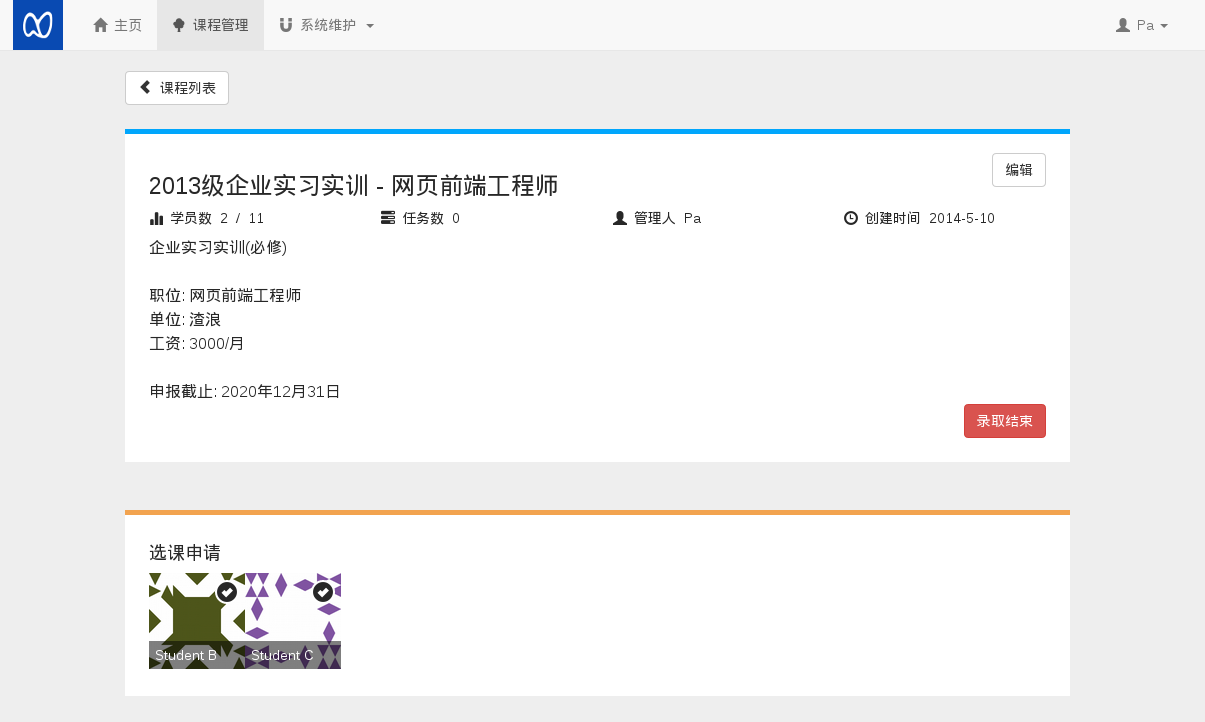
\includegraphics[scale=0.3]{figures/screenshot-enroll.png}
    \caption{学员录取视图\label{SSEnroll}}
  \end{center}
\end{figure}

\begin{figure}[!h]
  \begin{center}
    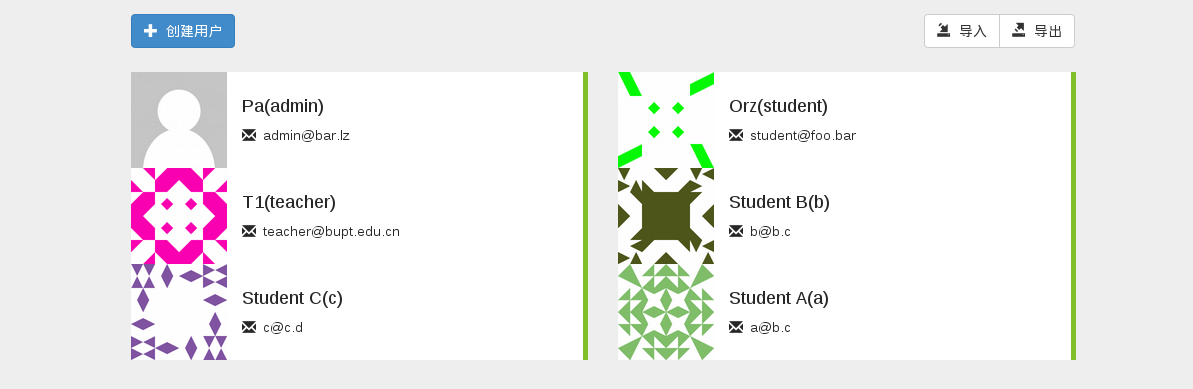
\includegraphics[scale=0.3]{figures/screenshot-usermgr.png}
    \caption{用户管理视图\label{SSUserMgr}}
  \end{center}
\end{figure}

\begin{figure}[!h]
  \begin{center}
    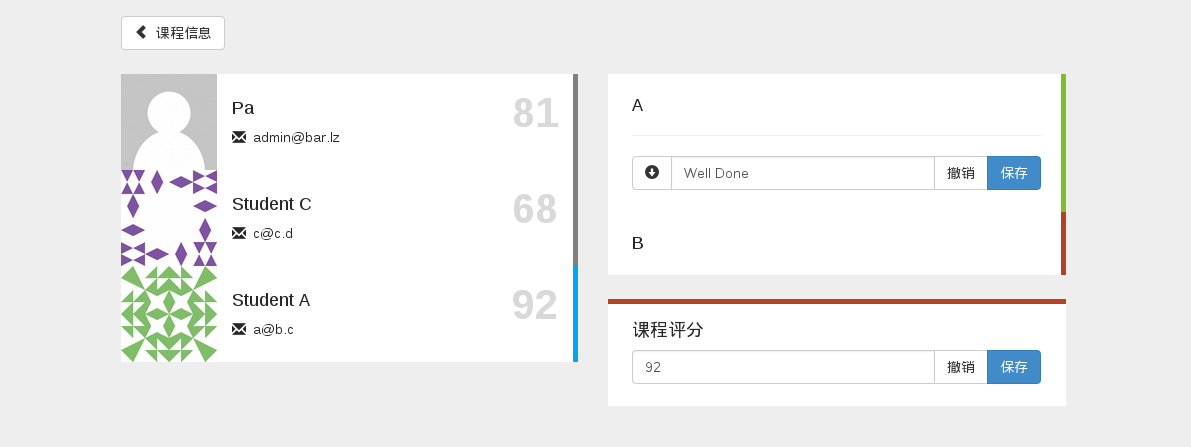
\includegraphics[scale=0.3]{figures/screenshot-course-review.png}
    \caption{课程评分视图\label{SSCourseReview}}
  \end{center}
\end{figure}

\begin{figure}[!h]
  \begin{center}
    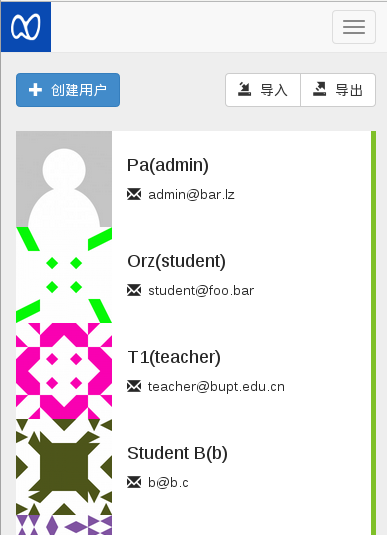
\includegraphics[scale=0.5]{figures/screenshot-responsive.png}
    \caption{用户管理视图(移动终端)\label{SSResponsive}}
  \end{center}
\end{figure}

